

Fast retrieval of similar patches is crucial for making
construction of a sizeable patch-based database feasible.
This is essentially near-neighbor retrieval in
relatively high dimensions $3 \cdot n^2$ (1875 for $n=25$).
Image retrieval has been addressed in a number of papers,
including more complex feature respresentations ~\cite{perronnin2010large}.
Our poblem is somewhat different from most of previous work
in that the variability
in small patches is much less than in regular-sized images,
and semantic information is irrelevant, and vectors are much shorter
than for regular-sized images.
Thus, we focus on tuning
a simple Locality-Sensitive Hashing variant for our
particular application.

\subsection{Locality-Sensitive Hashing}

Locality-Sensitive Hashing (LSH)~\cite{LSH:Andoni}
is popular approach to approximate near-neighbor search
in high dimensions.
Because this approach is hashing-based, it is
attractive for database applications, where entire lookup data structure
cannot be stored in memory.

At a high-level, LSH applies a family of hash functions $F_i$:

Why we don't want many hash tables:

\begin{equation*}
\begin{aligned}
P[b(P_i) = b(P_j) | S(P_i, P_j < T)] > P_1\\
P[b(P_i) = b(P_j) | S(P_i, P_j) > cT] < P_2
\end{aligned}
\end{equation*}

\begin{figure}[ht!]
\centering
\subfigure[Random projection hashing]{%
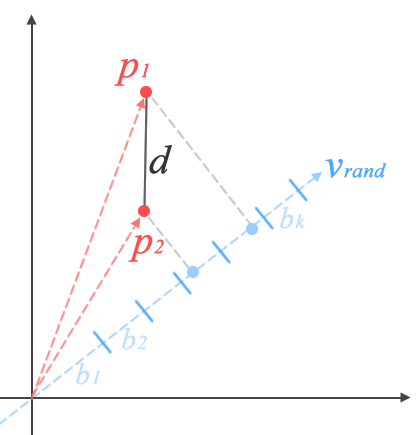
\includegraphics[width=1.5in]{fig_NN/rand_proj.png}
\label{fig:rand-proj}}
\quad
\subfigure[PCA-based hashing]{%
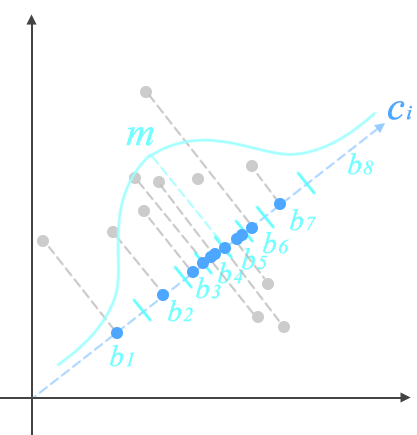
\includegraphics[width=1.5in]{fig_NN/pca_proj.png}
\label{fig:pca-proj}}
\caption{TODO.}
\label{fig:proj}
\end{figure}

\subsection{Naive LSH}

\subsection{PCA-based LSH}

\begin{figure}[ht!]
\centering
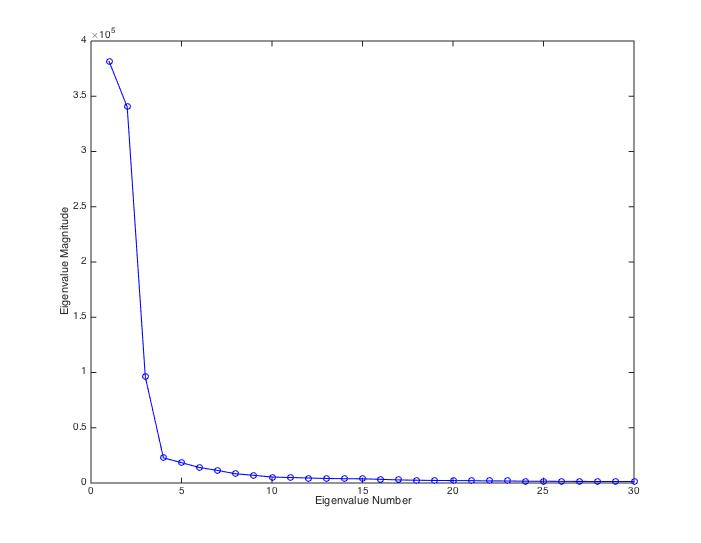
\includegraphics[width=3in]{fig_NN/lambdas.jpg}
\label{fig:lambdas}
\end{figure}

We ran Principal Component Analysis (PCA) on 80K patch vectors
sampled from 1000 images
sampled uinformly from all the categories in the
SUN database~\cite{SUN}.


\subsection{Self-similarity Optimization}

\subsection{Color Uniformity}

\subsection{Analysis}
